\documentclass[tikz,border=10pt]{standalone}
\usepackage{tikz}
\usetikzlibrary{shapes.geometric, arrows}

\tikzstyle{startstop} = [rectangle, rounded corners, minimum width=3cm, minimum height=1cm, text centered, draw=black, fill=red!30]
\tikzstyle{process} = [rectangle, minimum width=3cm, minimum height=1cm, text centered, draw=black, fill=blue!30]
\tikzstyle{arrow} = [thick,->,>=stealth]
\tikzstyle{note} = [text width=5cm, align=left]

\begin{document}
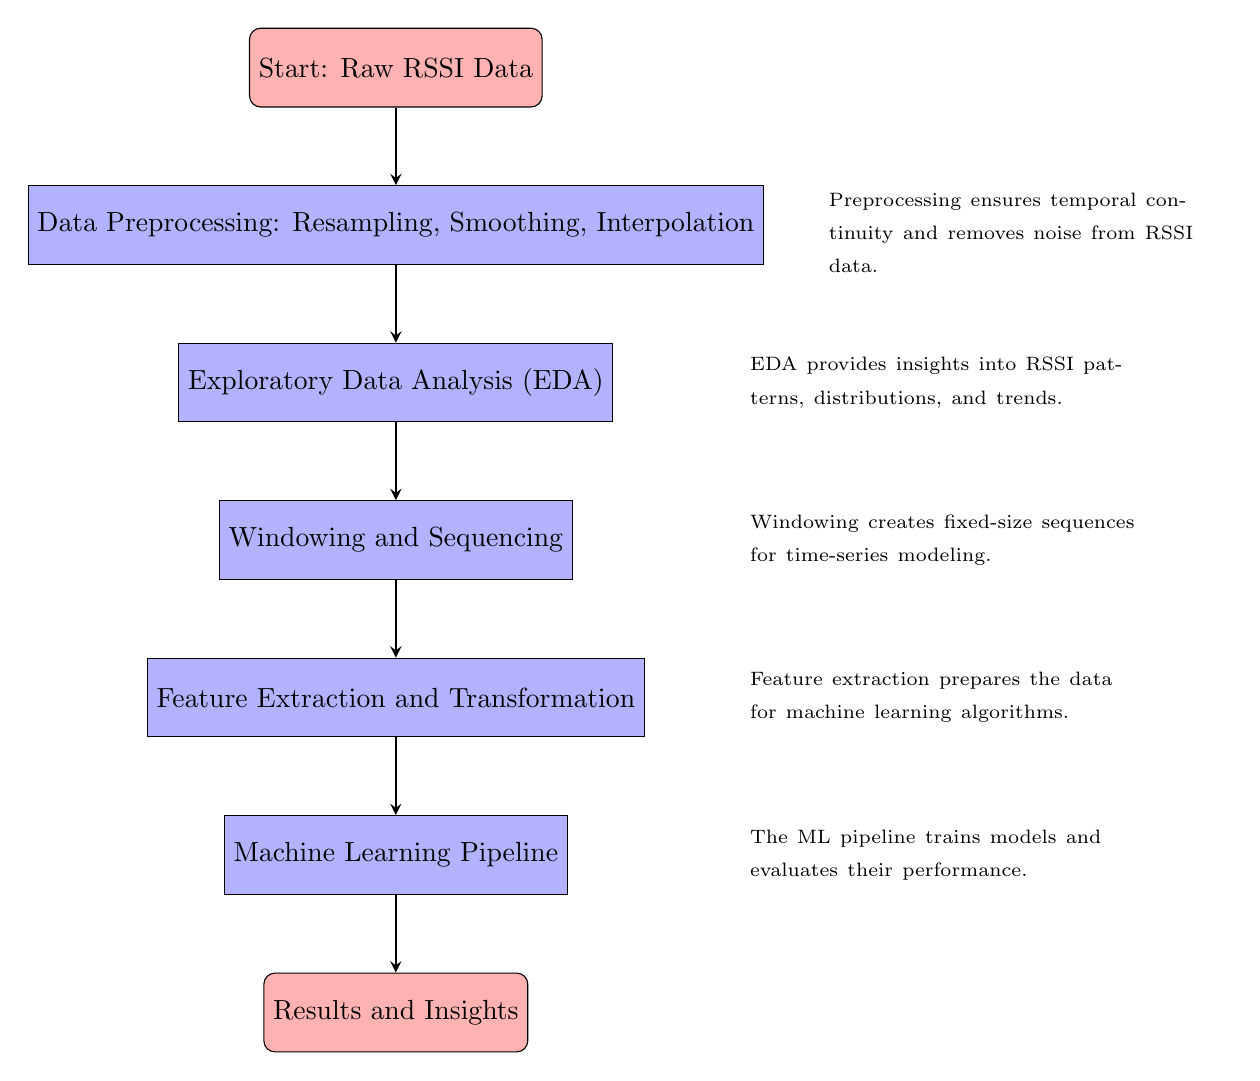
\begin{tikzpicture}[node distance=2cm]

% Nodes
\node (start) [startstop] {Start: Raw RSSI Data};
\node (preprocessing) [process, below of=start] {Data Preprocessing: Resampling, Smoothing, Interpolation};
\node (eda) [process, below of=preprocessing] {Exploratory Data Analysis (EDA)};
\node (windowing) [process, below of=eda] {Windowing and Sequencing};
\node (features) [process, below of=windowing] {Feature Extraction and Transformation};
\node (mlpipeline) [process, below of=features] {Machine Learning Pipeline};
\node (end) [startstop, below of=mlpipeline] {Results and Insights};

% Annotations
\node[note, right of=preprocessing, xshift=6 cm, yshift=-0.10cm] {\scriptsize Preprocessing ensures temporal continuity and removes noise from RSSI data.};
\node[note, right of=eda, xshift=5cm] {\scriptsize EDA provides insights into RSSI patterns, distributions, and trends.};
\node[note, right of=windowing, xshift=5cm] {\scriptsize Windowing creates fixed-size sequences for time-series modeling.};
\node[note, right of=features, xshift=5cm] {\scriptsize Feature extraction prepares the data for machine learning algorithms.};
\node[note, right of=mlpipeline, xshift=5cm] {\scriptsize The ML pipeline trains models and evaluates their performance.};

% Arrows
\draw [arrow] (start) -- (preprocessing);
\draw [arrow] (preprocessing) -- (eda);
\draw [arrow] (eda) -- (windowing);
\draw [arrow] (windowing) -- (features);
\draw [arrow] (features) -- (mlpipeline);
\draw [arrow] (mlpipeline) -- (end);

\end{tikzpicture}
\end{document}
